\section{Le pseudo-terminal}

\begin{frame}
	\begin{itemize}
		\item Permet une \textbf{communication asynchrone} et \textbf{bidirectionnelle} entre deux processus
		\item Une extrémité \textbf{maître} et une autre extrémité \textbf{esclave}
		
		\item Utilisé par les émulateurs de terminal, tels que \textit{konsole} sur KDE

		\item C'est le noyau qui se charge de la création des pseudo-terminaux

	\end{itemize}

	\begin{figure}
		\centering
		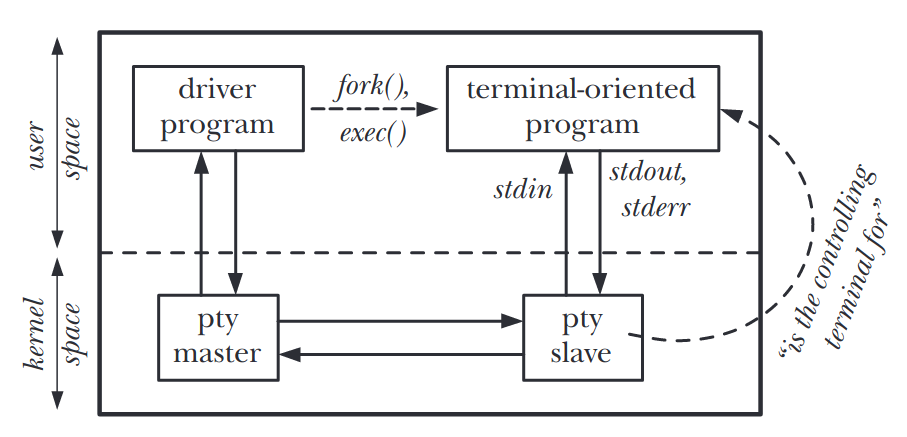
\includegraphics[width=5cm]{images/pseudo-terminal.png}
		\caption{Le fonctionnement du pseudo-terminal}
	\end{figure}
\end{frame}

\begin{frame}
	\begin{itemize}
		\item Un \textit{terminal de contrôle} pour les processus en \textit{foreground}

		\item Il gère les entrées, sorties et \textit{jobs} pour les pseudo-terminaux

		\item Une combinaison de touches permet de faire passer un processus en \textit{background}

			\begin{block}{Passer un processus en \textit{background}}
				Lorsqu'un processus s'exécute dans le shell Bash, on peut le basculer en arrière-plan en utilisant les touches \textit{CTRL+Z}. Pendant ce temps, le terminal reste disponible pour lancer d'autres commandes. Cette fonction est particulièrement utile pour des processus impliquant des tâches très longues.
			\end{block}
	\end{itemize}
\end{frame}

\begin{frame}
	\begin{itemize}
		\item Les processus se trouvent dans des \textit{sessions}
		\item Chaque session possède des groupes qui contiennent des processus
		\item Le groupes de processus dite \textit{foreground} détiennent le \textit{terminal de contrôle}
			\begin{figure}
				\centering
				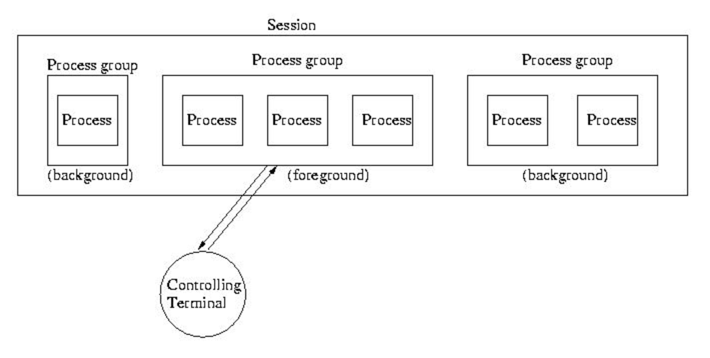
\includegraphics[width=6cm]{images/controlling_terminal.png}
				\caption{Les sessions \& groupes de processus sur Linux}
			\end{figure}
	\end{itemize}
\end{frame}
